\section{Einführung}
	\subsection{Ausbildungskernreaktor AKR-2}
	%TODO: Aufbau, technische Daten im Überblick (vgl erster Link http://tu-dresden.de/die_tu_dresden/fakultaeten/fakultaet_maschinenwesen/iet/wket/akr2/Lehrmaterialien)
	%TODO: Sicherheitsmechanismen (Wann kommt es zu einer RESA?
	\subsection{Kernspaltung}
	%TODO: Kernreaktion, Wirkungsquerschnitt für Neutroneneinfang von U-235 --> Warum benötigt man Moderator? Prompte/verzögerte Neutronen, Lebensdauer
	\subsection{Reaktorkinetik}
	%TODO: Multiplikationsfaktor k, Reaktivität, Reaktorperiode, Verdopplungszeit (nur nennen, nichts herleiten!)
	%TODO: Reaktorkinetische Gleichungen für überkritischen Reaktor + Lösungen --> Wie verhält sich Reaktorleistung bei Reaktivitätsänderung?
	
	\subsection{Steuerstabkalibrierung}
	%TODO: Gleichung für differentielle / integrale Steuerstabkennlinie, INHOUR-Gleichung, Gesamt-, Überschuss-, Abschaltreaktivität.
	Um die nukleare Sicherheit eines Kernreaktors jederzeit gewährleisten zu können, ist es wichtig, dass man weiß, wie sich die Neutronenbilanz im Reaktor unter Veränderung der vorhandenen Steuer- und Regeleinrichtungen verhält. Zu diesem Zweck bestimmt man die \textit{differentiellen} und \textit{integralen Steuerstabkennlinien} der vorliegenden Neutronenabsorber. \\
	Da die axiale Neutronenflussdichte $\Phi_z(z)$ eines zylindersymmetrischen Reaktors zum Rand der Spaltzone abnimmt, wird ein Steuerstab, der sich in der Mitte bewegt einen größeren Einfluss auf die Reaktivität haben als ein sich am Rand bewegender. Eine durch diesen Effekt erzeugte Reaktivitätsveränderung $\mathrm{d}\rho$ ist also proportional zur Neutronenflussdichte $\Phi_z(z)$, der Absorptionswahrscheinlichkeit der Neutronen am Absorber (Wechselwirkungsquerschnitt) $\Sigma_a$ und der eingeschobenen Länge $\mathrm{d}z$. Abbildung \ref{int:NeutrFlDichte} zeigt die ortsabhängige Neutronenflussdichteverteilung in der Spaltzone.\\
		\begin{figure}[hp]
			\centering
			\captionsetup{justification=centering}
			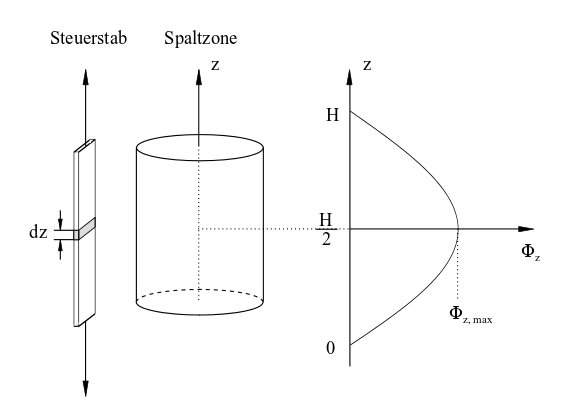
\includegraphics[scale=0.4]{pic/NeutrFlDichte}
			\caption{Zylindrische Spaltzone mit ortsabhängiger Neutronenflussdichte $\Phi_z(z)$}
			\label{int:NeutrFlDichte}
		\end{figure}
	\ \\
	Da Neutronen auch durch Oberflächenverluste ohne Absorption verloren gehen können, definiert man eine sogenannte \textit{Einflussfunktion} $f(z)$ , die beschreibt, wie groß der Einfluss der Neutronen am Ort $z$ auf die Reaktivität ist. Neutronen am Rand haben durch ihre höhere Verlustwahrscheinlichkeit einen geringeren Einfluss, weshalb die Einflussfunktion in etwa proptional zur Neutronendichte (welche zum Rand hin auch abnimmt) sein muss, d.h. $f(z) \propto \Phi_z(z)$. Überlagern wir diese beiden statistisch unabhängigen Effekte erhalten wir die \textit{differentielle Steuerstabkennlinie}:\\
	$$\frac{\mathrm{d}\rho}{\mathrm{d}z}(z) \propto \Sigma_a \cdot \Phi_z(z)$$
	Integrieren wir diese über eine makroskopische Länge z und normieren diese anschließend auf den Maximalwert $\rho_{max}$, erhalten wir die \textit{integrale Steuerstabkennlinie}:
	$$\frac{\rho(z)}{\rho_{max}} = \frac{z}{H} - \frac{1}{2\pi} \sin{\left(\frac{2\pi z}{H}\right)}$$
	Wobei H die effektive Länge der Spaltzone beschreibt. Abbildung zeigt den typischen Verlauf der Steuerstabkennlinien:
		\begin{figure}[hp]
				\centering
				\captionsetup{justification=centering}
				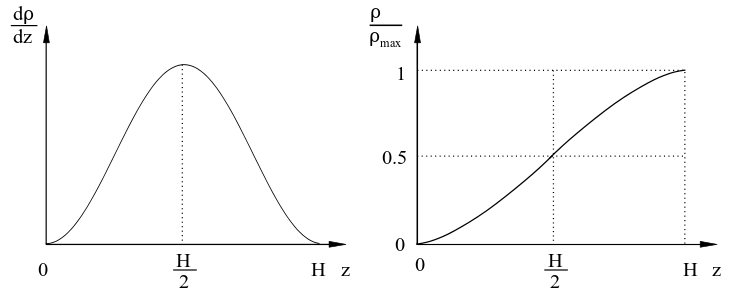
\includegraphics[scale=0.4]{pic/sskl}
				\caption{links: differentielle Steuerstabkennlinie, 
						\\rechts: integrale, auf Maximalwert normierte Steuerstabkennlinie}
				\label{int:NeutrFlDichte}
		\end{figure}
	\ \\
	
	